% Options for packages loaded elsewhere
\PassOptionsToPackage{unicode}{hyperref}
\PassOptionsToPackage{hyphens}{url}
\PassOptionsToPackage{dvipsnames,svgnames*,x11names*}{xcolor}
%
\documentclass[
  english,
  man,floatsintext]{apa6}
\usepackage{lmodern}
\usepackage{amssymb,amsmath}
\usepackage{ifxetex,ifluatex}
\ifnum 0\ifxetex 1\fi\ifluatex 1\fi=0 % if pdftex
  \usepackage[T1]{fontenc}
  \usepackage[utf8]{inputenc}
  \usepackage{textcomp} % provide euro and other symbols
\else % if luatex or xetex
  \usepackage{unicode-math}
  \defaultfontfeatures{Scale=MatchLowercase}
  \defaultfontfeatures[\rmfamily]{Ligatures=TeX,Scale=1}
\fi
% Use upquote if available, for straight quotes in verbatim environments
\IfFileExists{upquote.sty}{\usepackage{upquote}}{}
\IfFileExists{microtype.sty}{% use microtype if available
  \usepackage[]{microtype}
  \UseMicrotypeSet[protrusion]{basicmath} % disable protrusion for tt fonts
}{}
\makeatletter
\@ifundefined{KOMAClassName}{% if non-KOMA class
  \IfFileExists{parskip.sty}{%
    \usepackage{parskip}
  }{% else
    \setlength{\parindent}{0pt}
    \setlength{\parskip}{6pt plus 2pt minus 1pt}}
}{% if KOMA class
  \KOMAoptions{parskip=half}}
\makeatother
\usepackage{xcolor}
\IfFileExists{xurl.sty}{\usepackage{xurl}}{} % add URL line breaks if available
\IfFileExists{bookmark.sty}{\usepackage{bookmark}}{\usepackage{hyperref}}
\hypersetup{
  pdftitle={Epidemiologische situatie COVID-19 in Nederland - 28 november 2020},
  pdfauthor={Marino van Zelst1},
  pdflang={en-EN},
  colorlinks=true,
  linkcolor=Maroon,
  filecolor=Maroon,
  citecolor=Blue,
  urlcolor=blue,
  pdfcreator={LaTeX via pandoc}}
\urlstyle{same} % disable monospaced font for URLs
\usepackage{graphicx,grffile}
\makeatletter
\def\maxwidth{\ifdim\Gin@nat@width>\linewidth\linewidth\else\Gin@nat@width\fi}
\def\maxheight{\ifdim\Gin@nat@height>\textheight\textheight\else\Gin@nat@height\fi}
\makeatother
% Scale images if necessary, so that they will not overflow the page
% margins by default, and it is still possible to overwrite the defaults
% using explicit options in \includegraphics[width, height, ...]{}
\setkeys{Gin}{width=\maxwidth,height=\maxheight,keepaspectratio}
% Set default figure placement to htbp
\makeatletter
\def\fps@figure{htbp}
\makeatother
\setlength{\emergencystretch}{3em} % prevent overfull lines
\providecommand{\tightlist}{%
  \setlength{\itemsep}{0pt}\setlength{\parskip}{0pt}}
\setcounter{secnumdepth}{-\maxdimen} % remove section numbering
% Make \paragraph and \subparagraph free-standing
\ifx\paragraph\undefined\else
  \let\oldparagraph\paragraph
  \renewcommand{\paragraph}[1]{\oldparagraph{#1}\mbox{}}
\fi
\ifx\subparagraph\undefined\else
  \let\oldsubparagraph\subparagraph
  \renewcommand{\subparagraph}[1]{\oldsubparagraph{#1}\mbox{}}
\fi
% Manuscript styling
\usepackage{upgreek}
\captionsetup{font=singlespacing,justification=justified}

% Table formatting
\usepackage{longtable}
\usepackage{lscape}
% \usepackage[counterclockwise]{rotating}   % Landscape page setup for large tables
\usepackage{multirow}		% Table styling
\usepackage{tabularx}		% Control Column width
\usepackage[flushleft]{threeparttable}	% Allows for three part tables with a specified notes section
\usepackage{threeparttablex}            % Lets threeparttable work with longtable

% Create new environments so endfloat can handle them
% \newenvironment{ltable}
%   {\begin{landscape}\begin{center}\begin{threeparttable}}
%   {\end{threeparttable}\end{center}\end{landscape}}
\newenvironment{lltable}{\begin{landscape}\begin{center}\begin{ThreePartTable}}{\end{ThreePartTable}\end{center}\end{landscape}}

% Enables adjusting longtable caption width to table width
% Solution found at http://golatex.de/longtable-mit-caption-so-breit-wie-die-tabelle-t15767.html
\makeatletter
\newcommand\LastLTentrywidth{1em}
\newlength\longtablewidth
\setlength{\longtablewidth}{1in}
\newcommand{\getlongtablewidth}{\begingroup \ifcsname LT@\roman{LT@tables}\endcsname \global\longtablewidth=0pt \renewcommand{\LT@entry}[2]{\global\advance\longtablewidth by ##2\relax\gdef\LastLTentrywidth{##2}}\@nameuse{LT@\roman{LT@tables}} \fi \endgroup}

% \setlength{\parindent}{0.5in}
% \setlength{\parskip}{0pt plus 0pt minus 0pt}

% \usepackage{etoolbox}
\makeatletter
\patchcmd{\HyOrg@maketitle}
  {\section{\normalfont\normalsize\abstractname}}
  {\section*{\normalfont\normalsize\abstractname}}
  {}{\typeout{Failed to patch abstract.}}
\patchcmd{\HyOrg@maketitle}
  {\section{\protect\normalfont{\@title}}}
  {\section*{\protect\normalfont{\@title}}}
  {}{\typeout{Failed to patch title.}}
\makeatother
\shorttitle{Dagelijkse rapportage}
\DeclareDelayedFloatFlavor{ThreePartTable}{table}
\DeclareDelayedFloatFlavor{lltable}{table}
\DeclareDelayedFloatFlavor*{longtable}{table}
\makeatletter
\renewcommand{\efloat@iwrite}[1]{\immediate\expandafter\protected@write\csname efloat@post#1\endcsname{}}
\makeatother
\usepackage{csquotes}
\ifxetex
  % Load polyglossia as late as possible: uses bidi with RTL langages (e.g. Hebrew, Arabic)
  \usepackage{polyglossia}
  \setmainlanguage[]{english}
\else
  \usepackage[shorthands=off,main=english]{babel}
\fi

\title{Epidemiologische situatie COVID-19 in Nederland - 28 november 2020}
\author{Marino van Zelst\textsuperscript{1}}
\date{}


\affiliation{\vspace{0.5cm}\textsuperscript{1} Vragen over deze rapportage kunnen verstuurd worden aan Marino van Zelst, twitter.com/mzelst. E-mail: \href{mailto:j.m.vanzelst@uvt.nl}{\nolinkurl{j.m.vanzelst@uvt.nl}}}

\begin{document}
\maketitle

{
\hypersetup{linkcolor=}
\setcounter{tocdepth}{3}
\tableofcontents
}
\newpage

\hypertarget{samenvatting}{%
\section{Samenvatting}\label{samenvatting}}

\textbf{Samenvatting (op basis van GGD cijfers)}\\
Tot en met 2020-11-28 zijn er in Nederland in totaal 513325 COVID-19 patiënten gemeld aan het RIVM. Tot nu toe zijn 17493 van de gemelde patiënten opgenomen in het ziekenhuis en 9326 mensen overleden.

\textbf{Gegevens t. o. v. gisteren}\\
Positief getest: 4499
Totaal: 513325 (+ 4459 ivm -40 corr.)

Opgenomen: 71
Totaal: 17493 (+
69 ivm -2 corr.)

Opgenomen op IC: 6
Totaal: 5465

Overleden: 59
Totaal: 9326 (+
59 ivm 0 corr.)

\textbf{Update met betrekking tot ziekenhuis-gegevens (data NICE)}

Patiënten verpleegafdeling\\
Bevestigd: 10 Verdacht: 11

Patiënten IC\\
Bevestigd: 5 Verdacht: 1

\textbf{Data}\\
Een databestand met de cumulatieve aantallen per gemeente per dag van gemelde COVID-19 patiënten, in het ziekenhuis opgenomen COVID-19 patiënten en overleden COVID-19 patiënten is \href{https://data.rivm.nl/geonetwork/srv/dut/catalog.search\#/metadata/1c0fcd57-1102-4620-9cfa-441e93ea5604}{hier} te vinden. Een databestand met karakteristieken van elke positief geteste COVID-19 patiënt in Nederland is \href{https://data.rivm.nl/geonetwork/srv/dut/catalog.search\#/metadata/2c4357c8-76e4-4662-9574-1deb8a73f724?tab=relations}{hier} te vinden. Alle gegevens die voor dit rapport gebruikt worden zijn te vinden in de \href{https://github.com/mzelst/covid-19}{Github repository}.

\newpage

\hypertarget{covid-19-meldingen-in-de-afgelopen-vier-weken}{%
\section{COVID-19 meldingen in de afgelopen vier weken}\label{covid-19-meldingen-in-de-afgelopen-vier-weken}}

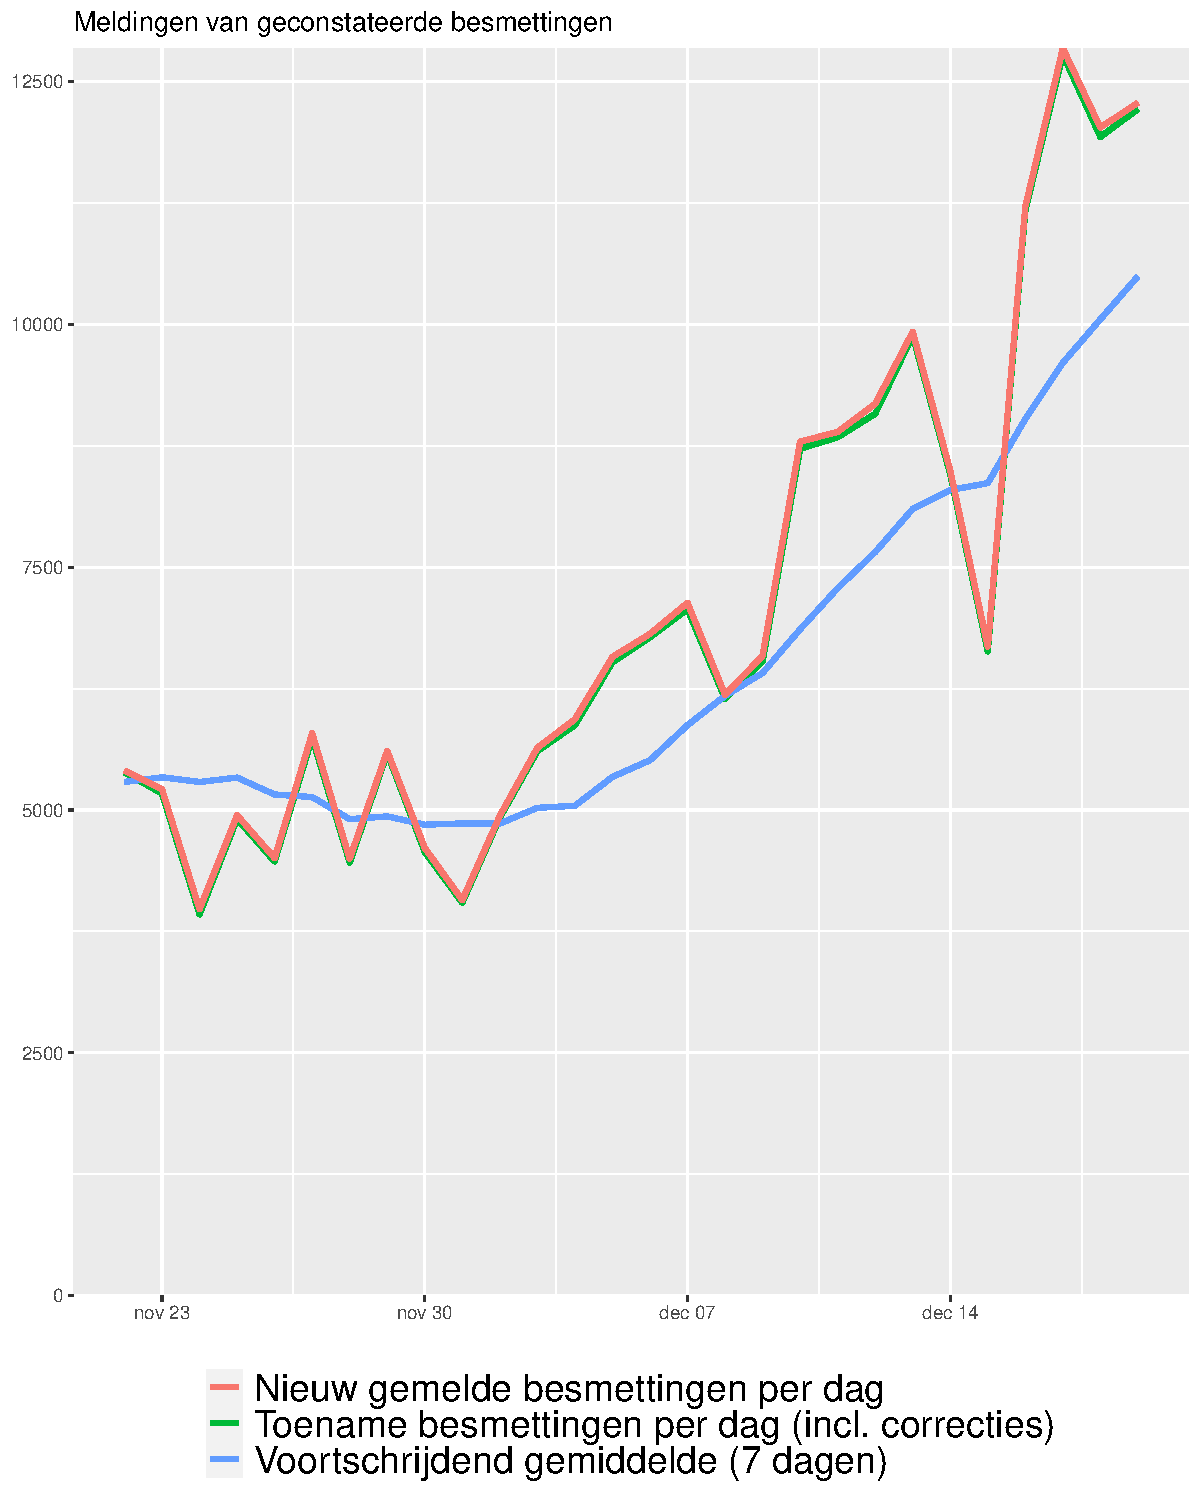
\includegraphics{daily_report_files/figure-latex/Gemelde besmettingen-1.pdf}

\newpage

\hypertarget{kaart-met-covid-19-meldingen-per-gemeente-sinds-gisteren}{%
\section{Kaart met COVID-19 meldingen per gemeente sinds gisteren}\label{kaart-met-covid-19-meldingen-per-gemeente-sinds-gisteren}}

\begin{figure}
\centering
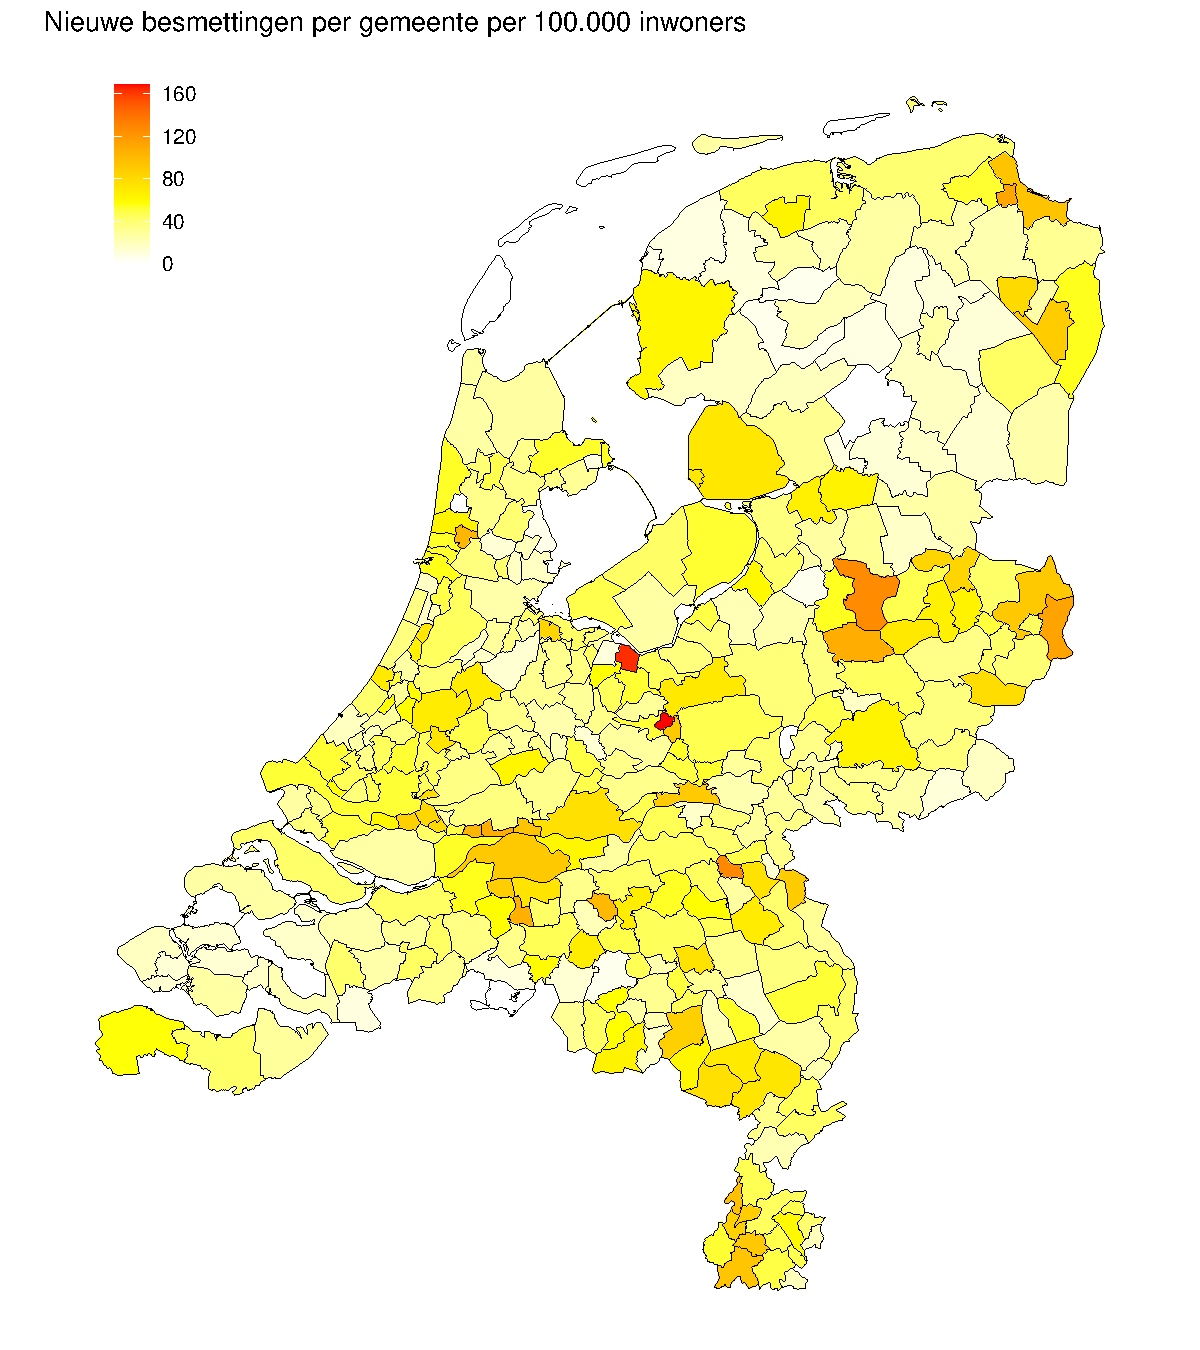
\includegraphics{daily_report_files/figure-latex/Gemeentes - sinds gisteren-1.pdf}
\caption{(\#Gemeentes - sinds gisteren) Aantal, sinds gisteren, bij de GGD'en gemelde COVID-19 patiënten per 100.000 inwoners per gemeente}
\end{figure}

\newpage

\hypertarget{kaart-met-covid-19-meldingen-per-gemeente-in-de-afgelopen-week}{%
\section{Kaart met COVID-19 meldingen per gemeente in de afgelopen week}\label{kaart-met-covid-19-meldingen-per-gemeente-in-de-afgelopen-week}}

\begin{figure}
\centering
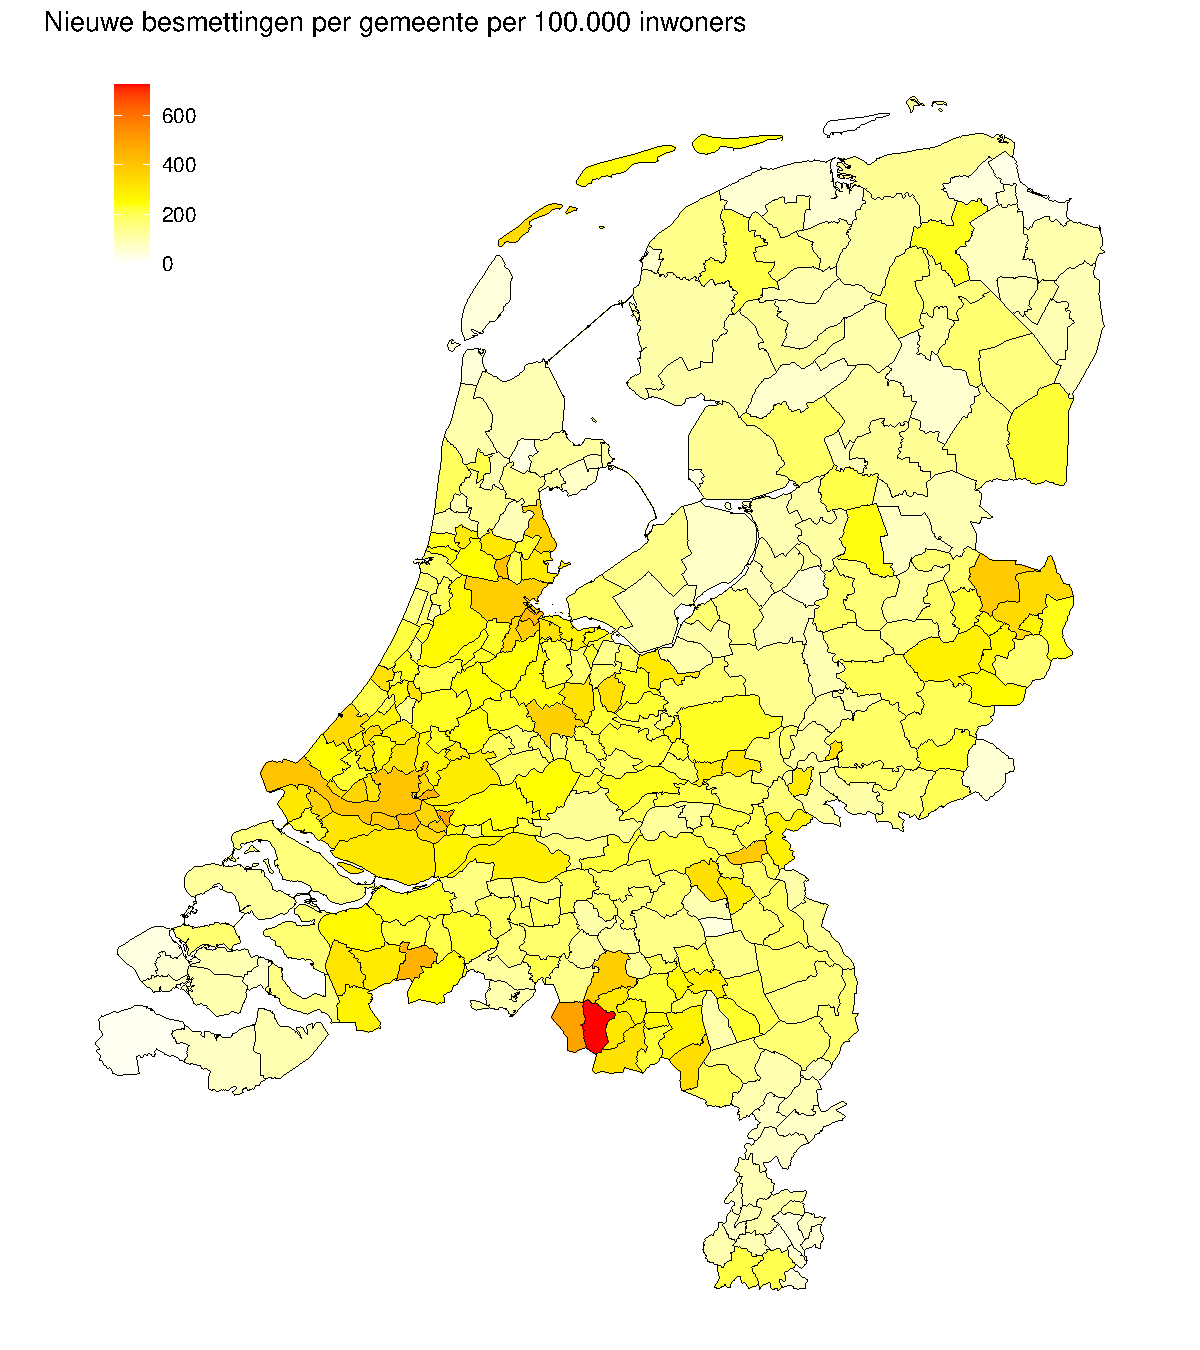
\includegraphics{daily_report_files/figure-latex/Gemeentes - Sinds vorige week-1.pdf}
\caption{(\#Gemeentes - Sinds vorige week) Aantal in de afgelopen week bij de GGD'en gemelde COVID-19 patiënten per 100.000 inwoners per gemeente.}
\end{figure}

\newpage

\hypertarget{aantal-covid-19-meldingen-per-provincie-in-de-afgelopen-twee-weken}{%
\section{Aantal COVID-19 meldingen per provincie in de afgelopen twee weken}\label{aantal-covid-19-meldingen-per-provincie-in-de-afgelopen-twee-weken}}

\begin{table}[H]
\centering
\begin{threeparttable}
\begin{tabular}{lrrrrrr}
\toprule
\multicolumn{1}{c}{ } & \multicolumn{2}{c}{Besmettingen} & \multicolumn{2}{c}{Ziekenhuisopnames} & \multicolumn{2}{c}{Overleden} \\
\cmidrule(l{3pt}r{3pt}){2-3} \cmidrule(l{3pt}r{3pt}){4-5} \cmidrule(l{3pt}r{3pt}){6-7}
Provincie & Totaal & /100000 & Totaal & /100000 & Totaal & /100000\\
\midrule
Drenthe & 1258 & 254.8 & 11 & 2.2 & 17 & 3.4\\
Flevoland & 2348 & 555.1 & 21 & 5.0 & 17 & 4.0\\
Friesland & 1402 & 215.7 & 19 & 2.9 & 29 & 4.5\\
Gelderland & 7746 & 371.3 & 79 & 3.8 & 103 & 4.9\\
Groningen & 1279 & 218.3 & 11 & 1.9 & 4 & 0.7\\
Limburg & 4066 & 363.9 & 37 & 3.3 & 40 & 3.6\\
Noord-Brabant & 12144 & 473.8 & 154 & 6.0 & 111 & 4.3\\
Noord-Holland & 11218 & 389.6 & 140 & 4.9 & 120 & 4.2\\
Overijssel & 4847 & 417.0 & 42 & 3.6 & 57 & 4.9\\
Utrecht & 5679 & 419.2 & 103 & 7.6 & 64 & 4.7\\
Zeeland & 1171 & 305.4 & 33 & 8.6 & 16 & 4.2\\
Zuid-Holland & 17709 & 477.5 & 436 & 11.8 & 305 & 8.2\\
\bottomrule
\end{tabular}
\begin{tablenotes}
\item \textit{Note: } 
\item Aantal bij de GGD’en gemelde COVID-19 patiënten, in het ziekenhuis opgenomen COVID-19 patiënten en overleden COVID-19 patiënten per provincie van 14 november t/m 28 november 10:00 uur, totaal en per 100.000 inwoners
\end{tablenotes}
\end{threeparttable}
\end{table}

\newpage

\hypertarget{aantal-covid-19-meldingen-per-ggd-in-de-afgelopen-twee-weken}{%
\section{Aantal COVID-19 meldingen per GGD in de afgelopen twee weken}\label{aantal-covid-19-meldingen-per-ggd-in-de-afgelopen-twee-weken}}

\begin{table}[H]
\centering\begingroup\fontsize{10}{12}\selectfont

\begin{threeparttable}
\begin{tabular}{lrrrrrr}
\toprule
\multicolumn{1}{c}{ } & \multicolumn{2}{c}{Besmettingen} & \multicolumn{2}{c}{Ziekenhuisopnames} & \multicolumn{2}{c}{Overleden} \\
\cmidrule(l{3pt}r{3pt}){2-3} \cmidrule(l{3pt}r{3pt}){4-5} \cmidrule(l{3pt}r{3pt}){6-7}
GGD & Totaal & /100000 & Totaal & /100000 & Totaal & /100000\\
\midrule
Dienst Gezondheid \& Jeugd ZHZ & 2331 & 510.2 & 12 & 2.6 & 25 & 5.5\\
GGD Amsterdam & 4495 & 424.8 & 81 & 7.7 & 51 & 4.8\\
GGD Brabant Zuid-Oost & 3516 & 454.7 & 49 & 6.3 & 27 & 3.5\\
GGD Drenthe & 1246 & 253.2 & 11 & 2.2 & 17 & 3.5\\
GGD Flevoland & 2351 & 564.4 & 22 & 5.3 & 16 & 3.8\\
GGD Fryslân & 1403 & 216.6 & 19 & 2.9 & 29 & 4.5\\
GGD Gelderland-Midden & 2833 & 410.5 & 15 & 2.2 & 26 & 3.8\\
GGD Gelderland-Zuid & 2232 & 394.7 & 28 & 5.0 & 32 & 5.7\\
GGD Gooi en Vechtstreek & 872 & 342.0 & 5 & 2.0 & 17 & 6.7\\
GGD Groningen & 1236 & 211.6 & 10 & 1.7 & 4 & 0.7\\
GGD Haaglanden & 4564 & 413.6 & 134 & 12.1 & 63 & 5.7\\
GGD Hart voor Brabant & 4984 & 467.9 & 58 & 5.4 & 54 & 5.1\\
GGD Hollands Midden & 3757 & 468.7 & 71 & 8.9 & 52 & 6.5\\
GGD Hollands Noorden & 2443 & 371.2 & 18 & 2.7 & 12 & 1.8\\
GGD IJsselland & 1539 & 291.9 & 18 & 3.4 & 15 & 2.8\\
GGD Kennemerland & 2051 & 376.0 & 19 & 3.5 & 15 & 2.8\\
GGD Limburg Noord & 2148 & 420.4 & 14 & 2.7 & 24 & 4.7\\
GGD Noord en Oost Gelderland & 2687 & 326.0 & 35 & 4.2 & 41 & 5.0\\
GGD Regio Twente & 3312 & 526.3 & 24 & 3.8 & 46 & 7.3\\
GGD regio Utrecht & 5660 & 421.7 & 102 & 7.6 & 63 & 4.7\\
GGD Rotterdam Rijnmond & 7144 & 544.5 & 220 & 16.8 & 167 & 12.7\\
GGD West Brabant & 3633 & 514.3 & 47 & 6.7 & 29 & 4.1\\
GGD Zaanstreek-Waterland & 1339 & 397.6 & 18 & 5.3 & 26 & 7.7\\
GGD Zeeland & 1170 & 305.5 & 33 & 8.6 & 16 & 4.2\\
GGD Zuid Limburg & 1921 & 321.6 & 23 & 3.9 & 16 & 2.7\\
\bottomrule
\end{tabular}
\begin{tablenotes}
\item \textit{Note: } 
\item Aantal bij de GGD’en gemelde COVID-19 patiënten, in het ziekenhuis opgenomen COVID-19 patiënten en overleden COVID-19 patiënten per GGD van 14 november t/m 28 november 10:00 uur, totaal en per 100.000 inwoners
\end{tablenotes}
\end{threeparttable}
\endgroup{}
\end{table}

\newpage

\hypertarget{leeftijdsverdeling-en-man-vrouwverdeling-van-covid-19-patiuxebnten-in-de-afgelopen-twee-weken}{%
\section{Leeftijdsverdeling en man-vrouwverdeling van COVID-19 patiënten in de afgelopen twee weken}\label{leeftijdsverdeling-en-man-vrouwverdeling-van-covid-19-patiuxebnten-in-de-afgelopen-twee-weken}}

\begin{table}[H]
\centering\begingroup\fontsize{11}{13}\selectfont

\begin{threeparttable}
\begin{tabular}{lrrrrrr}
\toprule
\multicolumn{1}{c}{ } & \multicolumn{2}{c}{Besmettingen} & \multicolumn{2}{c}{Ziekenhuisopnames} & \multicolumn{2}{c}{Overleden} \\
\cmidrule(l{3pt}r{3pt}){2-3} \cmidrule(l{3pt}r{3pt}){4-5} \cmidrule(l{3pt}r{3pt}){6-7}
Leeftijdsgroep & Totaal & \% & Totaal & \% & Totaal & \%\\
\midrule
0-9 & 864 & 1.2 & 19 & 1.8 & 0 & 0.0\\
10-19 & 11004 & 15.5 & 8 & 0.7 & 0 & 0.0\\
20-29 & 11146 & 15.7 & 20 & 1.8 & 0 & 0.0\\
30-39 & 10002 & 14.1 & 36 & 3.3 & 0 & 0.0\\
40-49 & 11117 & 15.7 & 48 & 4.4 & 0 & 0.0\\
50-59 & 11993 & 16.9 & 153 & 14.1 & 16 & 1.8\\
60-69 & 6859 & 9.7 & 227 & 20.9 & 55 & 6.3\\
70-79 & 4113 & 5.8 & 287 & 26.5 & 202 & 23.0\\
80-89 & 2794 & 3.9 & 237 & 21.9 & 402 & 45.8\\
90+ & 979 & 1.4 & 49 & 4.5 & 203 & 23.1\\
\bottomrule
\end{tabular}
\begin{tablenotes}
\item[1] Leeftijdsverdeling van bij de GGD’en gemelde COVID-19 patiënten, in het ziekenhuis opgenomen COVID-19 patiënten en overleden COVID-19 patiënten van 14 november t/m 28 november 10:00 uur.
\item[2] Let op: Het rapport wijkt op een punt af van de de wekelijkse RIVM rapportage. Het RIVM meldde in week 46 een sterfgeval in de leeftijdscategorie 15-19. Deze casus wordt niet gemeld in de casus dataset en dit overlijden is waarschijnlijk gemeld in de categorie '<50' (die we hier niet tonen).
\end{tablenotes}
\end{threeparttable}
\endgroup{}
\end{table}

\newpage

\begin{table}[H]
\centering\begingroup\fontsize{11}{13}\selectfont

\begin{threeparttable}
\begin{tabular}{lrrrrrr}
\toprule
\multicolumn{1}{c}{ } & \multicolumn{2}{c}{Besmettingen} & \multicolumn{2}{c}{Ziekenhuisopnames} & \multicolumn{2}{c}{Overleden} \\
\cmidrule(l{3pt}r{3pt}){2-3} \cmidrule(l{3pt}r{3pt}){4-5} \cmidrule(l{3pt}r{3pt}){6-7}
Geslacht & Totaal & \% & Totaal & \% & Totaal & \%\\
\midrule
Vrouw & 38159 & 53.8 & 430 & 39.6 & 412 & 46.7\\
Man & 32708 & 46.2 & 656 & 60.4 & 471 & 53.3\\
Onbekend & 0 & 0.0 & 0 & 0.0 & 0 & 0.0\\
\bottomrule
\end{tabular}
\begin{tablenotes}
\item \textit{Note: } 
\item Man-vrouwverdeling van bij de GGD’en gemelde COVID-19 patiënten, in het ziekenhuis opgenomen COVID-19 patiënten en overleden COVID-19 patiënten van 14 november t/m 28 november 10:00 uur.
\end{tablenotes}
\end{threeparttable}
\endgroup{}
\end{table}
\newpage


\end{document}
